% !TeX program = xelatex
% Compile with XeLaTeX. Keep fonts/ beside this file.
% The merged version additionally uses the original assets/ folder.
% Theme definitions and slide content are included here; no other .tex is required.
\documentclass[aspectratio=169,11pt]{beamer}
% Visual system and reusable TikZ helpers.
\usepackage{lmodern}
\usepackage{fontspec}
\usefonttheme{professionalfonts}
\setsansfont{NimbusSans-Regular.otf}[Path=fonts/,BoldFont=NimbusSans-Bold.otf,ItalicFont=NimbusSans-Italic.otf,BoldItalicFont=NimbusSans-BoldItalic.otf]
\newfontfamily\editorial{P052-Italic.otf}[Path=fonts/]
\usepackage{amsmath,amssymb,graphicx,tikz}
\usetikzlibrary{arrows.meta,calc,shapes.geometric,decorations.pathreplacing}
\setbeamertemplate{navigation symbols}{}
\setbeamertemplate{headline}{}
\setbeamertemplate{footline}{}
\setbeamertemplate{frametitle}{}
\setbeamersize{text margin left=0pt,text margin right=0pt}
\definecolor{charcoal}{HTML}{17201D}
\definecolor{ivory}{HTML}{F4F0E7}
\definecolor{forest}{HTML}{245842}
\definecolor{gold}{HTML}{D9B45E}
\definecolor{goldink}{HTML}{88631D}
\definecolor{sage}{HTML}{A8C1AE}
\definecolor{muted}{HTML}{6B766D}
\definecolor{rulegray}{HTML}{D5D9CE}
\definecolor{softgreen}{HTML}{E4EADF}
\definecolor{softgold}{HTML}{EEE1BF}
\definecolor{stone}{HTML}{9DADA2}
\newcommand{\Dark}{\colorlet{bg}{charcoal}\colorlet{fg}{ivory}\colorlet{accent}{gold}\colorlet{subtle}{sage}\colorlet{linecol}{forest}}
\newcommand{\Light}{\colorlet{bg}{ivory}\colorlet{fg}{charcoal}\colorlet{accent}{forest}\colorlet{subtle}{muted}\colorlet{linecol}{rulegray}}
\newenvironment{canvas}{\begin{tikzpicture}[remember picture,overlay]\begin{scope}[shift={(current page.north west)},x=1cm,y=-1cm]\fill[bg] (0,0) rectangle (16,9);}{\end{scope}\end{tikzpicture}}
\hyphenpenalty=10000
\exhyphenpenalty=10000
\newcommand{\T}[6]{\pgfmathsetmacro{\leading}{#4*1.15}\node[anchor=north west,inner sep=0pt,align=left,text width=#3cm,text=#5,font=\fontsize{#4}{\leading}\selectfont] at (#1,#2) {#6};}
\newcommand{\C}[5]{\node[anchor=center,inner sep=0pt,text=#4,font=\fontsize{#3}{#3}\selectfont] at (#1,#2) {#5};}
\newcommand{\Header}[2]{\T{.8}{.52}{14}{7}{accent}{\textbf{#1}}\T{.8}{1.03}{14.4}{22}{fg}{\textbf{#2}}}
\newcommand{\Footer}[1]{\draw[linecol,line width=.35pt] (.8,8.39)--(15.2,8.39);\T{.8}{8.56}{12.9}{5.5}{subtle}{#1}\T{14.5}{8.52}{.7}{7}{subtle}{\textbf{\insertframenumber}\,/\,\inserttotalframenumber}}
\newcommand{\Play}[3]{\fill[#3] (#1,#2) circle (.20);\fill[ivory] ({#1-.055},{#2-.09})--({#1-.055},{#2+.09})--({#1+.105},#2)--cycle;}
\newcommand{\Thumb}[5]{\begin{scope}\clip (#2,#3) rectangle ({#2+#4},{#3+#5});\node[anchor=north west,inner sep=0pt] at ({#2-(#1-1)*#4},{#3-(#4-#5)/2}) {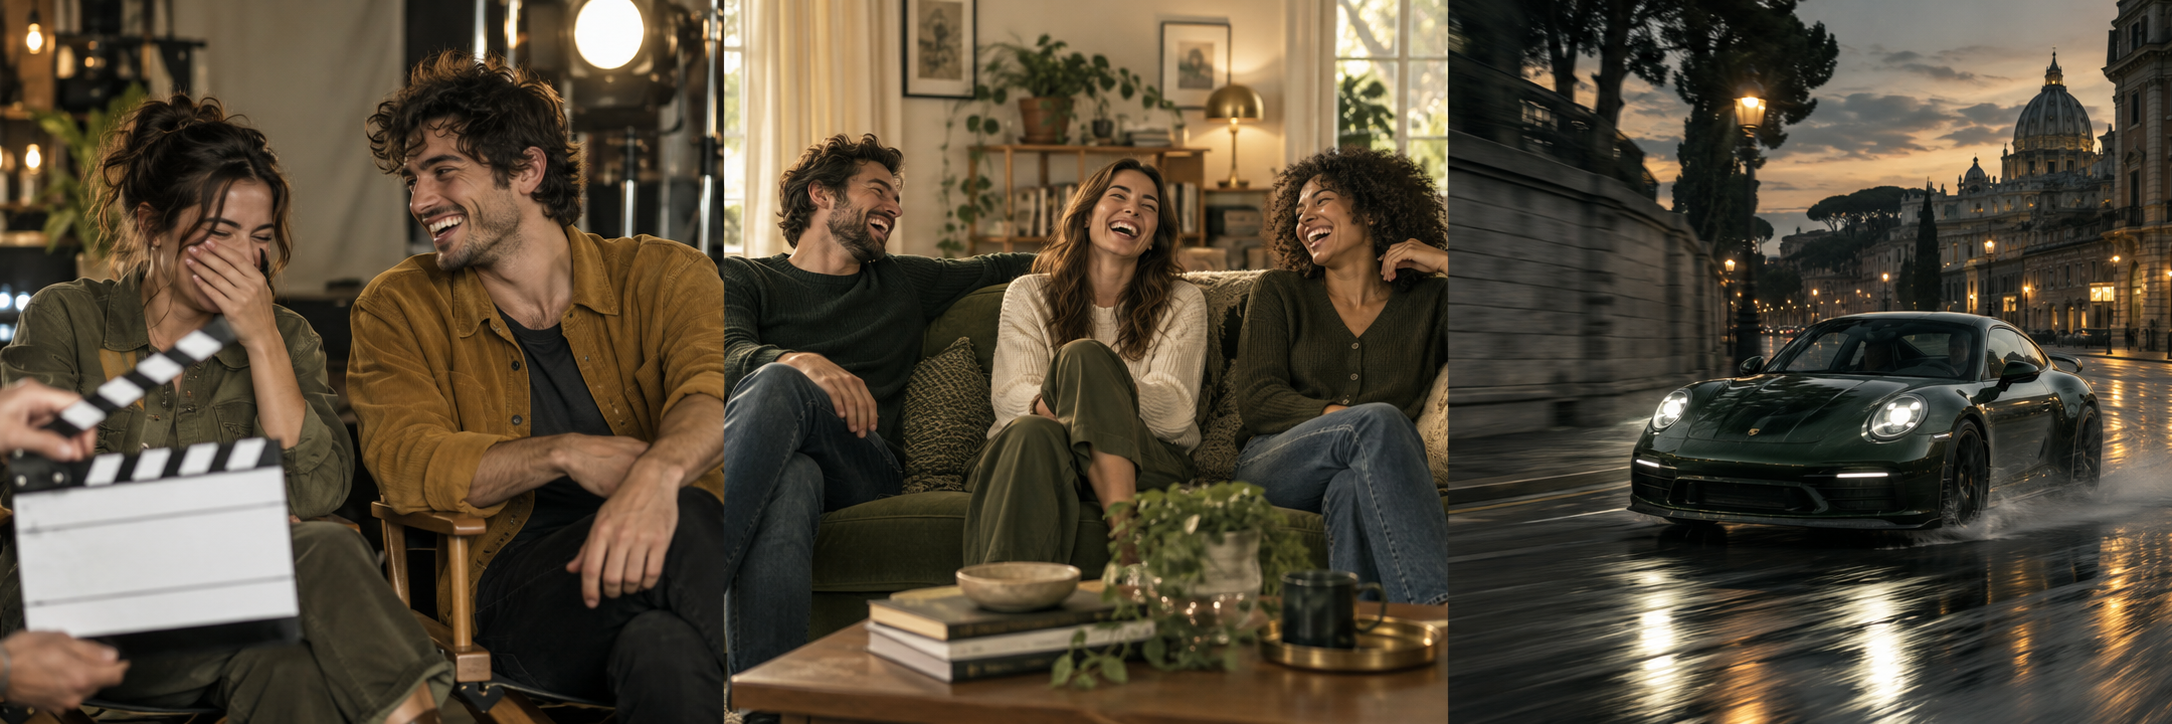
\includegraphics[width=\dimexpr#4cm*3\relax]{assets/videos.png}};\end{scope}}
\newcommand{\Force}[1]{\only<#1>{\relax}}
\title{Recommendation Algorithms: Bob's Next Video}
\author{Sami}
\date{}
\hypersetup{pdftitle={Recommendation Algorithms | Sami | Speaker 1},pdfauthor={Sami},pdfsubject={Feedback, user-item matrix, and content-based filtering},pdfpagemode=FullScreen}

% ---------- Adapter for the supplied continuation ----------
% Colors and helpers are local to each frame, so Sami's frames remain intact.
\usepackage{bm,booktabs,array,adjustbox}
\usetikzlibrary{positioning,fit,matrix,overlay-beamer-styles}
\newsavebox{\PartContent}
\newsavebox{\PartTitle}
\newcommand{\PartSectionOffset}{0}
\newcommand{\PartSectionNumber}{%
  \ifnum\numexpr\insertframenumber-\PartSectionOffset\relax<10 0\fi
  \number\numexpr\insertframenumber-\PartSectionOffset\relax}
\newcommand{\PartPalette}[1]{%
  \csname #1\endcsname
  \colorlet{ink}{fg}\colorlet{muted}{subtle}%
  \colorlet{blue}{accent}\colorlet{cyan}{accent}%
  \colorlet{teal}{forest}\colorlet{amber}{goldink}%
  \colorlet{rose}{goldink}\colorlet{violet}{forest}%
  \colorlet{paleBlue}{softgreen}\colorlet{paleTeal}{softgreen}%
  \colorlet{paleAmber}{softgold}\colorlet{paleRose}{softgold}%
  \colorlet{paleViolet}{softgreen}\colorlet{panel}{bg}%
  \ifstrequal{#1}{Dark}{%
    \colorlet{teal}{sage}\colorlet{amber}{gold}%
    \colorlet{rose}{gold}\colorlet{violet}{sage}%
    \colorlet{paleBlue}{forest}\colorlet{paleTeal}{forest}%
    \colorlet{paleAmber}{charcoal!78!gold}%
    \colorlet{paleRose}{charcoal!78!gold}%
    \colorlet{paleViolet}{forest}%
  }{}%
  \color{fg}%
}
\newcommand{\PartHeader}[2]{%
  \T{.8}{.52}{14}{7}{accent}{\textbf{#1}}%
  \node[anchor=north west,inner sep=0pt,text=fg]
    at (.8,1.03) {\begin{adjustbox}{max width=14.4cm}\usebox{\PartTitle}\end{adjustbox}};%
}
\newcommand{\PartStart}[4]{%
  \PartPalette{#1}%
  \sbox{\PartTitle}{{\normalfont\sffamily\bfseries\fontsize{22}{25.3}\selectfont #3}}%
  \begin{canvas}
    \PartHeader{#2}{#3}
    \Footer{#4}
  \end{canvas}%
}
% Same bold Nimbus hierarchy as the reference; no extra font dependency.
\newcommand{\textbfPro}[1]{{\sffamily\bfseries\fontsize{12}{14}\selectfont #1}}
\newcommand{\micro}[1]{{\fontsize{8}{10}\selectfont\textcolor{subtle}{#1}}}
\newcommand{\callout}[3][]{%
  \begin{center}\begin{tikzpicture}
    \node[rectangle,draw=accent,fill=paleBlue,text=fg,line width=.7pt,
      inner xsep=10pt,inner ysep=7pt,text width=#2,align=left,
      font=\fontsize{11}{13.2}\selectfont,#1]
      {\hyphenpenalty=10000\relax#3\par};
  \end{tikzpicture}\end{center}%
}
\tikzset{
  box/.style={rectangle,draw=linecol,fill=panel,text=fg,align=center,
    inner sep=7pt,font=\fontsize{11}{13.2}\selectfont,line width=.7pt},
  boxblue/.style={box,draw=blue,fill=paleBlue},
  boxteal/.style={box,draw=teal,fill=paleTeal},
  boxamber/.style={box,draw=amber,fill=paleAmber},
  boxrose/.style={box,draw=rose,fill=paleRose},
  boxviolet/.style={box,draw=violet,fill=paleViolet},
  user/.style={circle,draw=forest,fill=forest,text=ivory,
    minimum size=7mm,inner sep=0pt,font=\fontsize{9}{10}\selectfont\bfseries,line width=.8pt},
  item/.style={circle,draw=goldink,fill=gold,text=charcoal,
    minimum size=7mm,inner sep=0pt,font=\fontsize{9}{10}\selectfont\bfseries,line width=.8pt},
  feat/.style={circle,draw=forest,fill=sage,text=charcoal,
    minimum size=7mm,inner sep=0pt,font=\fontsize{9}{10}\selectfont\bfseries,line width=.8pt},
  arr/.style={line width=1.1pt,draw=accent},
  greyarr/.style={line width=.8pt,draw=subtle},
  dashedarr/.style={line width=1.1pt,draw=rose,dashed}
}
% Place the original content between the fixed reference header and footer.
% Invisible overlay objects still reserve their space.
\newenvironment{PartBody}{%
  \begin{lrbox}{\PartContent}\begin{minipage}{14.4cm}
    \color{fg}\sffamily\fontsize{11}{13.2}\selectfont
    \setlength{\parindent}{0pt}%
}{%
  \end{minipage}\end{lrbox}%
  \begin{tikzpicture}[remember picture,overlay]
    \node[anchor=center,inner sep=0pt,text=fg]
      at ([yshift=-5.15cm]current page.north)
      {\begin{adjustbox}{max totalsize={14.4cm}{5.7cm}}\usebox{\PartContent}\end{adjustbox}};
  \end{tikzpicture}%
}

\hypersetup{pdftitle={Collaborative filtering and recommendation algorithms},pdfauthor={Presentation team},pdfsubject={Recommendation algorithms}}
\begin{document}

% Continuation frame 1: original text and reveals retained.
\begin{frame}[plain]
\PartStart{Light}{\PartSectionNumber\ / COLLABORATIVE FILTERING}{Collaborative filtering}{2305033 - collaborative}
\begin{PartBody}
\centering
\begin{tikzpicture}
\node[user] (u1) at (2,3.8) {U1}; \node[user] (u2) at (2,2.75) {U2}; \node[user] (u3) at (2,1.7) {U3}; \node[user] (u4) at (2,.65) {U4};
\node[item] (m1) at (7,4.15) {M1}; \node[item] (m2) at (7,3.1) {M2}; \node[item] (m3) at (7,2.05) {M3}; \node[item] (m4) at (7,1.0) {M4};
\draw[greyarr,visible on=<1->] (u1)--(m1); \draw[greyarr,visible on=<1->] (u1)--(m2); \draw[greyarr,visible on=<1->] (u2)--(m1); \draw[greyarr,visible on=<1->] (u2)--(m2); \draw[greyarr,visible on=<1->] (u3)--(m3); \draw[greyarr,visible on=<1->] (u4)--(m4);
\draw[dashedarr,visible on=<2->] (u1)--node[above,sloped,font=\scriptsize,text=rose]{predict}(m3);
\node[boxteal,text width=4.1cm,visible on=<3->] at (11.2,2.4) {\textbfPro{Collaborative signal}\\If users with similar histories liked $M_3$, estimate that $U_1$ may also like $M_3$.};
\end{tikzpicture}
\end{PartBody}
\end{frame}

% Continuation frame 2: original text and reveals retained.
\begin{frame}[plain]
\PartStart{Light}{\PartSectionNumber\ / TWO FAMILIES}{Collaborative filtering has two main families}{2305033 - two families}
\begin{PartBody}
\centering
\begin{tikzpicture}
\node[boxteal,text width=5.8cm,visible on=<1->] (r) at (6.7,5.3) {\textbfPro{Shared evidence}\\sparse user--item matrix $R$};
\node[boxblue,text width=5.4cm,minimum height=3.0cm,visible on=<2->] (mem) at (3.25,2.35) {\textbfPro{Memory-based}\\[3pt]Use $R$ directly\\Find similar users or items\\Predict from neighbours\\[3pt]\micro{User-KNN \textbullet\ Item-KNN}};
\node[boxviolet,text width=5.4cm,minimum height=3.0cm,visible on=<3->] (model) at (10.15,2.35) {\textbfPro{Model-based}\\[3pt]Learn parameters from $R$\\Compress users and items\\Predict from learned vectors\\[3pt]\micro{Matrix factorization \textbullet\ SVD}};
\draw[arr,visible on=<2->] (r.south west)--(mem.north);
\draw[arr,visible on=<3->] (r.south east)--(model.north);
\node[boxamber,text width=12.6cm,visible on=<4->] at (6.7,0.0) {\textbfPro{Same evidence:} neighbours now, or learned structure first.};
\end{tikzpicture}
\end{PartBody}
\end{frame}

% Continuation frame 3: original text and reveals retained.
\begin{frame}[plain]
\PartStart{Dark}{\PartSectionNumber\ / MEMORY-BASED METHODS}{Memory-based methods}{2305033 - memory based}
\begin{PartBody}
\centering
\begin{tikzpicture}
\node[user] (target) at (6,2.7) {U};
\foreach \x/\y/\n in {4.3/3.9/A,4.8/1.55/B,7.25/3.6/C,7.8/1.6/D,5.9/4.2/E}{\node[user] (u\n) at (\x,\y) {\n};}
\draw[dashedarr,visible on=<2->] (target)--(uA); \draw[dashedarr,visible on=<2->] (target)--(uB);
\draw[greyarr,visible on=<3->] (uA)--(8.15,2.56); \draw[greyarr,visible on=<3->] (uB)--(8.15,2.56);
\node[item,visible on=<3->] (m) at (8.15,2.56) {M};
\node[boxblue,text width=3cm,visible on=<1->] at (1.6,2.55) {\textbfPro{User-based}\\find users similar to target user};
\node[boxteal,text width=3cm,visible on=<1->] at (10.8,3.25) {\textbfPro{Item-based}\\find items similar to target item};
\node[boxteal,text=ink,line width=.7pt,anchor=north,text width=12cm,visible on=<4->] at (6.5,.9) {Prediction comes from observed neighbours, without first learning a latent representation.};
\end{tikzpicture}
\end{PartBody}
\end{frame}

% Continuation frame 4: original text and reveals retained.
\begin{frame}[plain]
\PartStart{Light}{\PartSectionNumber\ / LIMITATIONS}{Why memory-based methods struggle at scale}{2305033 - limitations}
\begin{PartBody}
\centering
\begin{tikzpicture}[node distance=.75cm]
\node[boxrose,text width=2.9cm,visible on=<1->] (s) {\textbfPro{Sparsity}\\two users may overlap on very few items};
\node[boxamber,text width=3.2cm,right=of s,visible on=<2->] (scale) {\textbfPro{Scalability}\\similarity over millions of users/items is expensive};
\node[boxviolet,text width=3.2cm,right=of scale,visible on=<3->] (partial) {\textbfPro{Preference is partial}\\a click does not always mean preference};
\node[boxteal,text width=4.6cm,below=1.1cm of scale,visible on=<4->] (sol) {\textbfPro{Model-based direction}\\Learn a compact model once, then reuse it for prediction.};
\draw[arr,visible on=<4->] (s)--(sol); \draw[arr,visible on=<4->] (scale)--(sol); \draw[arr,visible on=<4->] (partial)--(sol);
\end{tikzpicture}
\end{PartBody}
\end{frame}

% Continuation frame 5: original text and reveals retained.
\begin{frame}[plain]
\PartStart{Light}{\PartSectionNumber\ / MATRIX FORMULATION}{Model-based matrix formulation}{2305033 - model formulation}
\begin{PartBody}
\centering
\begin{tikzpicture}
\node[boxrose,inner sep=6pt,visible on=<1->] (r) at (2.4,2.75) {\begin{tabular}{ccccc}5&?&4&?&1\\?&4&?&5&?\\4&?&?&4&2\\?&1&2&?&4\\5&?&?&?&4\end{tabular}};
\node[font=\LARGE\bfseries,text=blue,visible on=<2->] at (5.0,2.75) {$\approx$};
\node[boxblue,inner sep=6pt,visible on=<2->] (p) at (7.1,2.75) {\begin{tabular}{ccc}.6&.1&.8\\.7&.2&.7\\.1&.9&.9\\.9&.1&.1\\.2&.7&.8\end{tabular}};
\node[font=\LARGE\bfseries,text=blue,visible on=<2->] at (8.9,2.75) {$\times$};
\node[boxteal,inner sep=6pt,visible on=<2->] (q) at (11.4,2.75) {\begin{tabular}{ccccc}.9&.5&.7&.8&.2\\.1&.8&.2&.9&.3\\.5&.1&.8&.9&.3\end{tabular}};
\node[boxteal,text=ink,line width=.7pt,anchor=north,text width=11.8cm,visible on=<3->] at (7,1.15) {Learn $P$ and $Q$ so that $p_u^\top q_i$ matches known values in $R$ and predicts the missing ones.};
\end{tikzpicture}
\end{PartBody}
\end{frame}

% Continuation frame 6: original text and reveals retained.
\begin{frame}[plain]
\PartStart{Dark}{\PartSectionNumber\ / LATENT FEATURES}{Model-based latent features}{2305033 - model representation}
\begin{PartBody}
\centering
\begin{tikzpicture}
\node[boxrose,text width=2.0cm,visible on=<1->] (r) at (1.6,3.1) {\textbfPro{Large sparse matrix}\\$m\times n$\\mostly unknown};
\node[boxblue,text width=2.0cm,visible on=<2->] (p) at (5.1,3.1) {\textbfPro{User matrix}\\$P$\\$m\times k$};
\node[boxteal,text width=2.0cm,visible on=<2->] (q) at (8.4,3.1) {\textbfPro{Item matrix}\\$Q^\top$\\$k\times n$};
\draw[arr,visible on=<2->] (r)--(p); \draw[arr,visible on=<2->] (p)--(q);
\node[boxamber,text width=3.2cm,visible on=<3->] at (11.8,2.7) {{\editorial\fontsize{14}{16}\selectfont Why possible?}\\User preferences are not random; they contain reusable patterns.};
\node[boxteal,text=ink,line width=.7pt,anchor=north,text width=10.8cm,visible on=<4->] at (6.5,.55) {The model may discover axes such as ``mainstream vs niche'' or ``light comedy vs dark drama'' without human labels.};
\end{tikzpicture}
\end{PartBody}
\end{frame}

% Continuation frame 7: original text and reveals retained.
\begin{frame}[plain]
\PartStart{Light}{\PartSectionNumber\ / NEAREST NEIGHBOURS}{KNN predicts from nearest neighbours}{2305052 - KNN}
\begin{PartBody}
\begin{columns}[T,onlytextwidth]
\column{.45\textwidth}
\centering
\begin{tikzpicture}[scale=.93]
\node[user] (t) at (2.3,2.6) {T};
\node[user] (a) at (1.2,3.6) {A}; \node[user] (b) at (3.6,3.35) {B}; \node[user] (c) at (1.0,1.7) {C}; \node[user] (d) at (3.7,1.35) {D};
\draw[dashedarr,visible on=<2->] (t)--(a); \draw[dashedarr,visible on=<2->] (t)--(b); \draw[dashedarr,visible on=<2->] (t)--(c);
\node[boxviolet,visible on=<2->] at (2.35,.35) {$k=3$ neighbors};
\end{tikzpicture}
\column{.55\textwidth}
\visible<3->{\callout[draw=violet!55,fill=paleViolet,align=center]{6.5cm}{\textbfPro{Weighted prediction}\\[3pt]$\displaystyle \hat r_{ui}=\bar r_u+\frac{\sum_{v\in N(u)}s(u,v)(r_{vi}-\bar r_v)}{\sum_{v\in N(u)} |s(u,v)|}$}}
\vspace{.15cm}
\visible<4->{\small The neighborhood provides local evidence, usually measured by cosine or Pearson similarity.}
\end{columns}
\end{PartBody}
\end{frame}

% Continuation frame 8: original text and reveals retained.
\begin{frame}[plain]
\PartStart{Light}{\PartSectionNumber\ / COSINE SIMILARITY}{Cosine similarity compares vector direction}{2305052 - similarity}
\begin{PartBody}
\centering
\begin{tikzpicture}[>={Latex[length=2.5mm]}]
\draw[->,draw=ink!45] (1,1) -- (11.7,1) node[right]{Movie 1};
\draw[->,draw=ink!45] (1,1) -- (1,4.7) node[above]{Movie 2};
\draw[->,line width=1.4pt,draw=blue] (1,1) -- (8.3,4.25) node[above]{\small $x_u$};
\draw[->,line width=1.4pt,draw=stone] (1,1) -- (6.9,2.55) node[above]{\small $x_v$};
\draw[->,line width=1.4pt,draw=rose] (1,1) -- (9.0,1.55) node[right]{\small $x_w$};
\node[boxblue,visible on=<2->] at (10.8,3.7) {$\displaystyle \cos(\theta)=\frac{x_u^\top x_v}{\lVert x_u\rVert\lVert x_v\rVert}$};
\node[boxteal,visible on=<3->] at (3.35,3.55) {small angle};
\node[boxrose,visible on=<4->] at (5.3,0.45) {larger angle};
\end{tikzpicture}
\end{PartBody}
\end{frame}

% Continuation frame 9: original text and reveals retained.
\begin{frame}[plain]
\PartStart{Dark}{\PartSectionNumber\ / LATENT FACTORS}{SVD learns latent factors}{2305052 - SVD}
\begin{PartBody}
\centering
\begin{tikzpicture}
\node[boxrose,text width=2.0cm,visible on=<1->] at (0.3,3.15) {\textbfPro{Observed}\\$R$\\$m\times n$};
\node[font=\LARGE\bfseries,text=blue,visible on=<2->] at (2.15,3.15) {$\approx$};
\node[boxblue,text width=1.5cm,visible on=<2->] at (3.75,3.15) {$U_k$\\$m\times k$};
\node[boxamber,text width=1.5cm,visible on=<2->] at (5.98,3.15) {$\Sigma_k$\\$k\times k$};
\node[boxteal,text width=1.5cm,visible on=<2->] at (8.15,3.15) {$V_k^\top$\\$k\times n$};
\node[boxviolet,text width=2.15cm,visible on=<3->] at (10.79,3.15) {\textbfPro{Prediction}\\$\hat r_{ui}=p_u^\top q_i$};
\node[boxviolet,text=ink,line width=.7pt,anchor=north,text width=10.4cm,visible on=<4->] at (6.4,1.48) {$\displaystyle \min_{P,Q}\sum_{(u,i)\in\Omega}(r_{ui}-p_u^\top q_i)^2+\lambda(\lVert p_u\rVert^2+\lVert q_i\rVert^2)$};

\end{tikzpicture}
\end{PartBody}
\end{frame}

% Continuation frame 10: original text and reveals retained.
\begin{frame}[plain]
\PartStart{Light}{\PartSectionNumber\ / RECOMMENDER WORKFLOW}{End-to-end recommender workflow}{2305052 - workflow}
\begin{PartBody}
\centering
\begin{tikzpicture}
\node[boxblue,visible on=<1->] (a) at (0.5,3.25) {Sparse data};
\node[boxteal,visible on=<2->] (b) at (2.9,3.25) {Train\\\micro{SGD / ALS}};
\node[boxamber,visible on=<3->] (c) at (5.69,3.25) {Latent vectors\\$P,Q$};
\node[boxviolet,visible on=<4->] (d) at (8.39,3.25) {Predict\\$\hat r_{ui}$};
\node[boxrose,visible on=<5->] (e) at (10.33,3.25) {Rank\\top-$N$};
\draw[arr,visible on=<2->] (a)--(b); \draw[arr,visible on=<3->] (b)--(c); \draw[arr,visible on=<4->] (c)--(d); \draw[arr,visible on=<5->] (d)--(e);
\node[boxblue,text width=2.75cm,visible on=<6->] at (0.75,1.25) {\textbfPro{KNN}\\Explainable, weaker at scale};
\node[boxteal,text width=2.75cm,visible on=<6->] at (5.12,1.25) {\textbfPro{MF / SVD}\\Compressed latent factors};
\node[boxviolet,text width=3.05cm,visible on=<6->] at (9.5,1.25) {\textbfPro{Modern systems}\\Hybrid: content + collaborative};
\end{tikzpicture}
\end{PartBody}
\end{frame}

% Continuation frame 11: original text and reveals retained.
\begin{frame}[plain]
\PartStart{Dark}{\PartSectionNumber\ / TAKEAWAYS}{Takeaways}{Conclusion}
\begin{PartBody}
\centering
\begin{tikzpicture}
\node[boxblue,text width=2.65cm,visible on=<1->] (a) at (0.45,2.7) {\textbfPro{Sparse matrix}\\Observed only partially.};
\node[boxteal,text width=2.65cm,visible on=<2->] (b) at (4.10,2.7) {\textbfPro{Two families}\\Content + collaborative.};
\node[boxamber,text width=2.65cm,visible on=<3->] (c) at (7.65,2.7) {\textbfPro{Scaling idea}\\Compress into latent factors.};
\node[boxrose,text width=2.65cm,visible on=<4->] (d) at (11.17,2.7) {\textbfPro{Final output}\\Ranked personalized choices.};
\end{tikzpicture}
\vspace{.35cm}
\visible<5->{\callout[draw=violet!55,fill=paleViolet]{11.6cm}{The system does not know exactly what we will like; it estimates from patterns shared across users, items and context.\par\vspace{2pt}{\scriptsize\textcolor{ink!75}{References: LearnOpenCV guide, supplied PowerPoint/PDF outline, supplied YouTube transcript.}\par}}}
\end{PartBody}
\end{frame}

\end{document}
